\chapter{Background on Raman Spectroscopy}
\label{ch:background}

This chapter reviews the domain background for this work. Section~\ref{sec:rs_fundamentals} describes the physics of Raman Spectroscopy (RS); Section~\ref{sec:rs_medical} surveys its use in medical diagnostics; Section~\ref{sec:glioma_grading} addresses the current state of glioma tumour grading, the challenges associated with it, and the origin of the methylation classes used as labels throughout this work; and Section~\ref{sec:synthetic_rs} surveys approaches to synthetic data generation and augmentation for RS. The mathematical background for the specific methods used in this work is deferred to Chapter~\ref{ch:theory}.

\section{Raman Spectroscopy Fundamentals}
\label{sec:rs_fundamentals}
Raman Spectroscopy (RS) is a molecular fingerprinting technique that relies on light scattering properties of molecules to identify the chemical composition of a sample. \cite{Jones2019} It has many applications in materials science, chemistry, and biology, and has been shown to be a promising tool for medical diagnostics. \cite{shen2026advances,stupak2025raman} In particular, RS has been used to identify cancerous tissue in various organs, including the brain. \cite{Auner2018}

A comprehensive and systematic approach to the Raman phenomenon can be found in the book The Raman Effect by Derek A. Long. \cite{Long2002} We will present here only a simplified physics model of light matter interaction to explain the effect, as presented in the first chapter of the book. 

Raman Spectroscopy works by shining a laser light on a sample and measuring the scattered light. Light scattering refers to the pattern of light interaction with matter. We will assume that the sample that is probed is an "assembly of freely rotating, non-interacting molecules" \cite{Long2002}.

A laser emits light at a single angular frequency $\omega_1$. When such light touches a molecular system, most light either passes through or is scattered without change in frequency. This scattering without change of frequency is called elastic scattering or Rayleigh scattering. However, in experiments, pairs of other frequencies were observed at $\omega_s = \omega_1 \pm \omega_M$, where $\omega_s$ denotes the scattered frequency and $\omega_M$ a frequency corresponding to a transition between two molecular energy levels. This scattering with change of frequency is called Raman scattering. The collection of frequencies with the amplitude of the scattering are called a Raman spectrum. One such frequency is referred to as a Raman band. Bands at lower frequencies than the incident light, that is scattered frequencies for which the light lost energy, are called Stokes bands. In practice, it has been observed that bands with greater frequency appear as well, as mentioned before, in pairs with the Stokes frequencies, albeit at much lower intensity. Those bands are called anti-Stokes bands. Stokes formulated the law in the context of light fluorescence, postulating that fluorescent light has lower frequency that incident light. The terminology reflects whether the scattered light respects Stokes law or contradict it.

\begin{figure}[h]
    \centering
    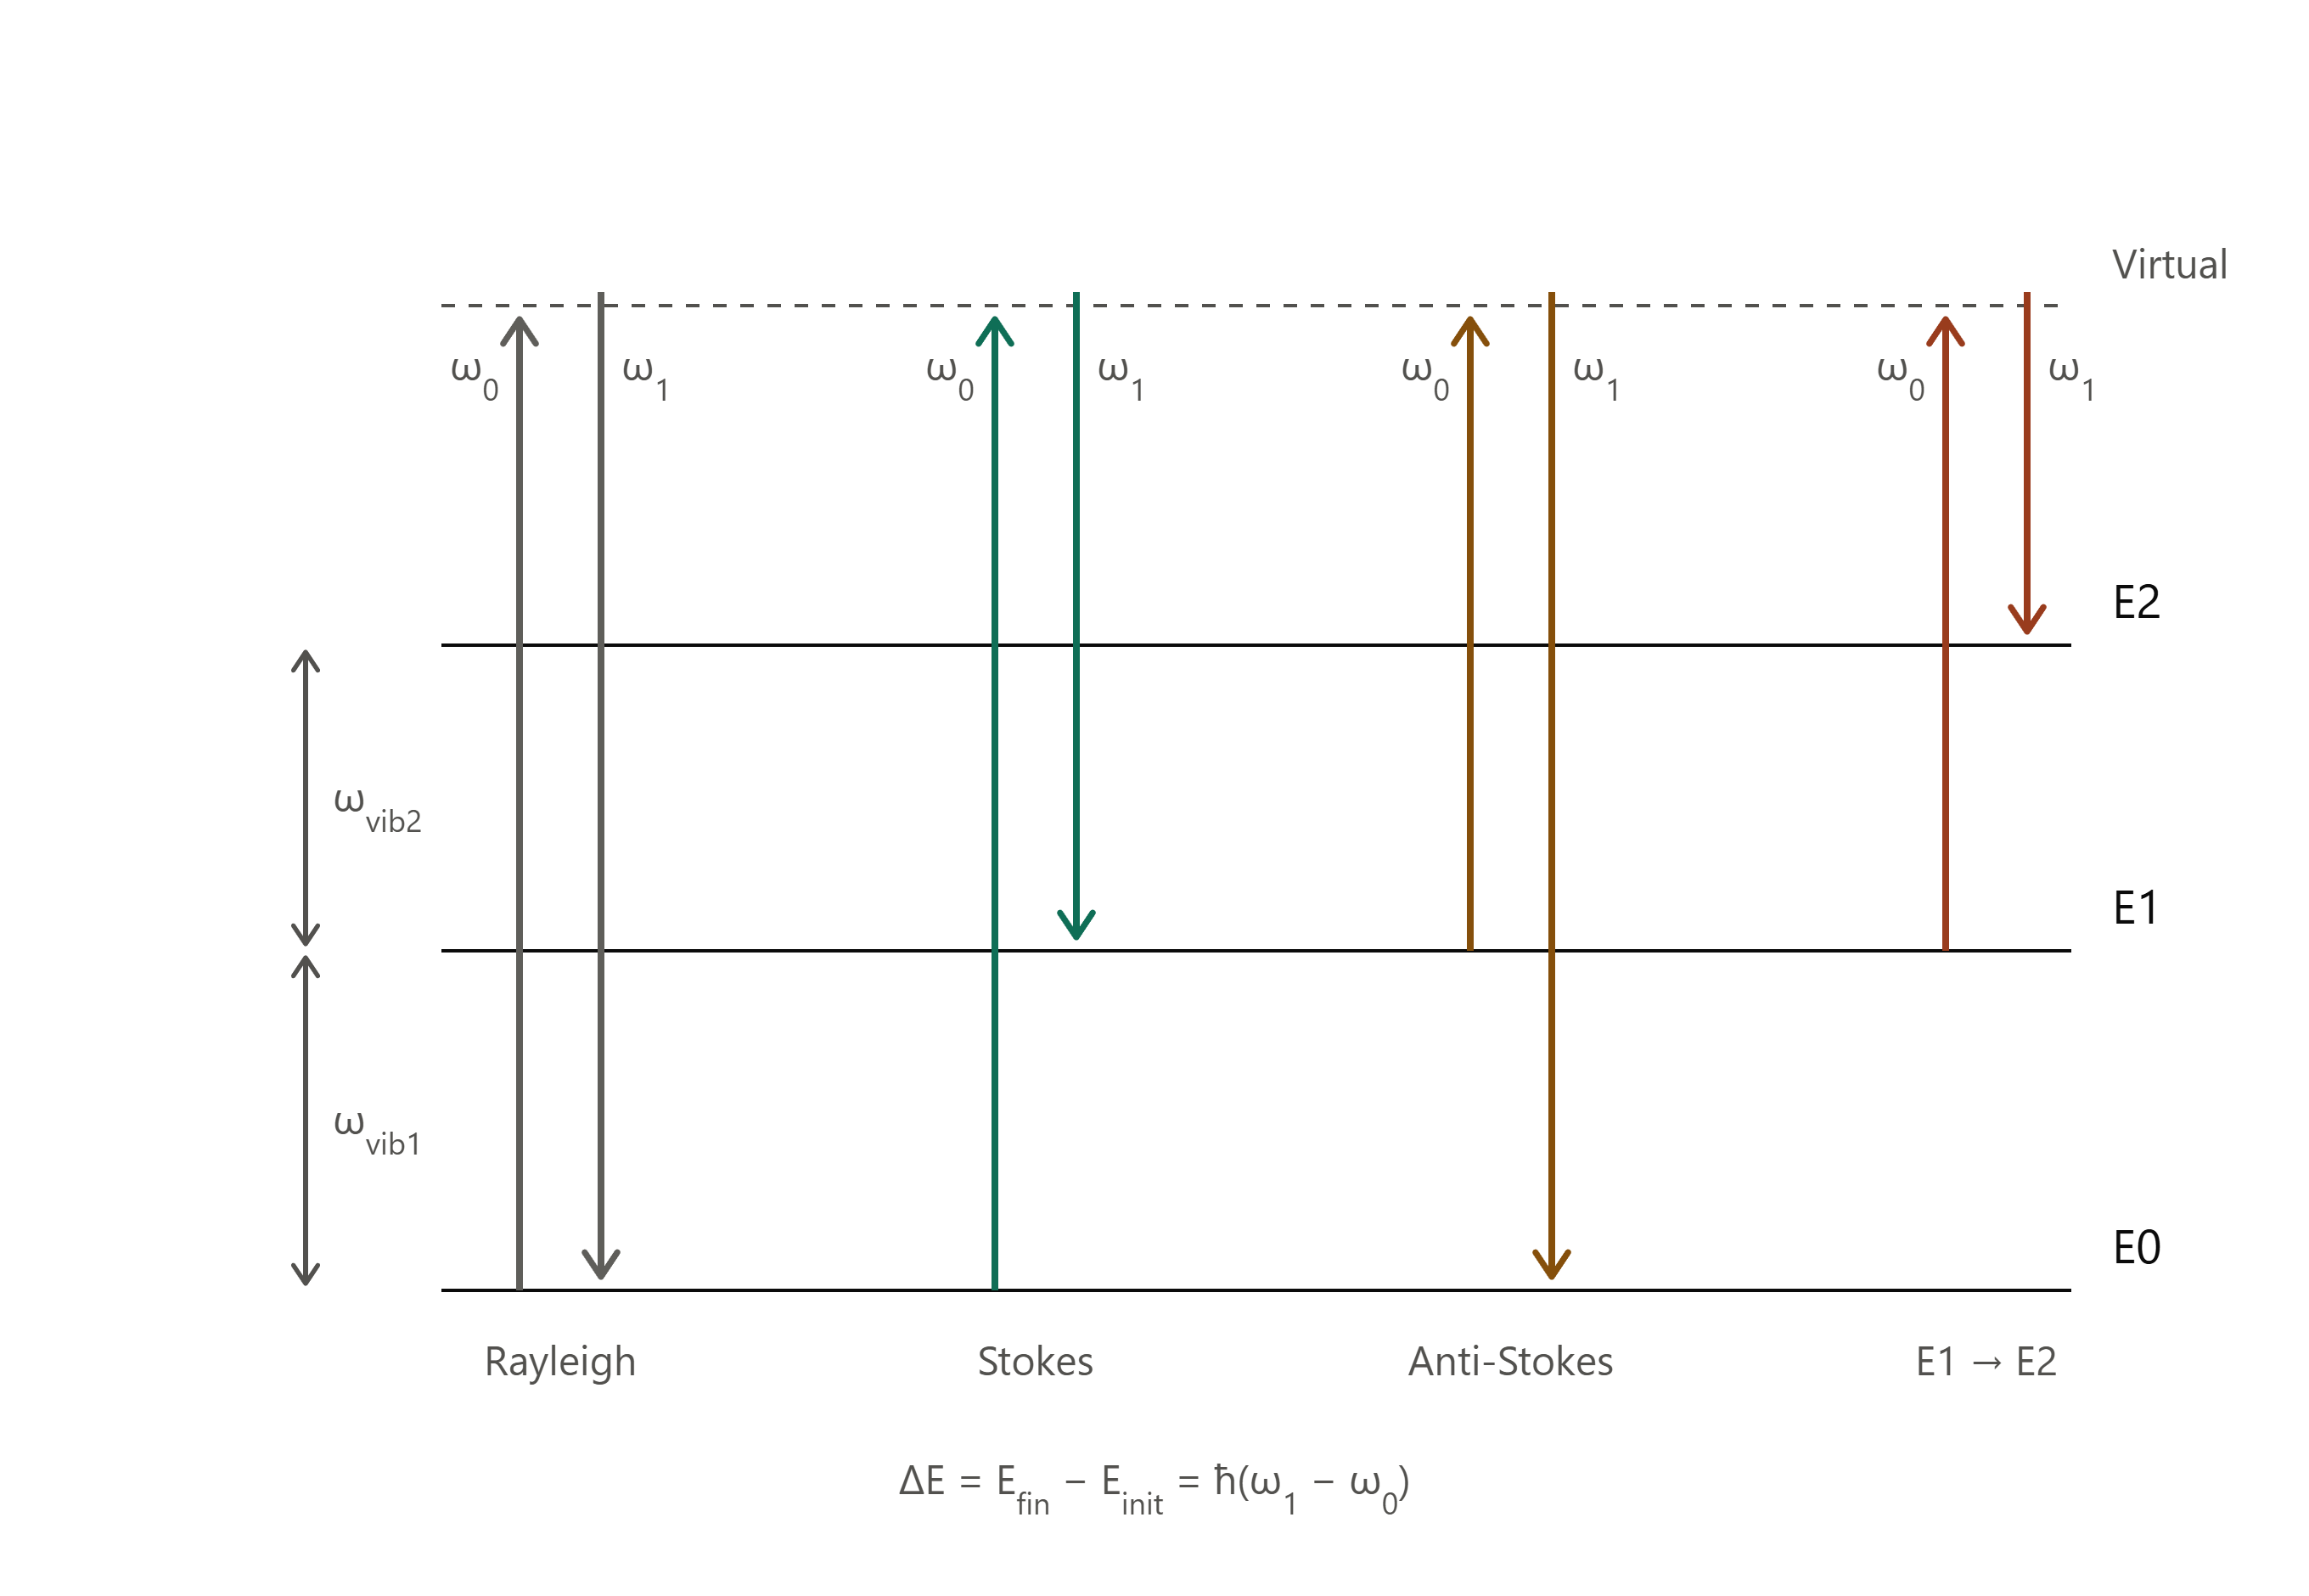
\includegraphics[width=\linewidth]{images/rayleigh_raman_energy_diagram.png}
    \caption{\footnotesize Diagram of energy model of the molecule-photon system.}
    \label{fig:energy_diagram}
\end{figure}

To understand the phenomenon let's consider a model of the energy of the system. Let's consider a very simple system with only one molecule and one photon. In figure \ref{fig:energy_diagram} we can see how the energy is transfered between the molecule and the photon. We know that energy states of molecules are discrete \cite{steinfeld2012molecules}, therefore changes in energy level of the molecule can only happen at precise quantities corresponding to the difference in energy levels. In the case of Rayleigh scattering, the molecular energy $E_{init} = E_{fin}$, and the incident and scattered photons have the same frequency, $\omega_s = \omega_1$. In the case of Raman scattering the molecular energy changes by $\Delta E = E_{fin}-E_{init} = \hbar ( \omega_1 - \omega_s)$, which is positive for Stokes scattering ($\omega_s < \omega_1$, the molecule gains energy) and negative for anti-Stokes scattering ($\omega_s > \omega_1$). Note that in all cases, the total energy of the photon-molecule system is preserved throughout this interaction.

Other types of light scattering exists and do happen in the course of performing Raman Spectroscopy. For example, at high incident intensities a molecule can scatter two photons at once, producing weak bands near $2\omega_1 \pm \omega_M$. This phenomenon is called hyper-Raman scattering. Another important phenomenon that interacts with the Raman signal is fluorescence, which manifests across larger band regions. We will address those issues when we deal with processing the signal. For illustration purposes, Figure \ref{fig:raw_spectrum} represents one raman spectrum from our dataset of Raman spectra of glioma biopsies.

\begin{figure}[h]
    \centering
    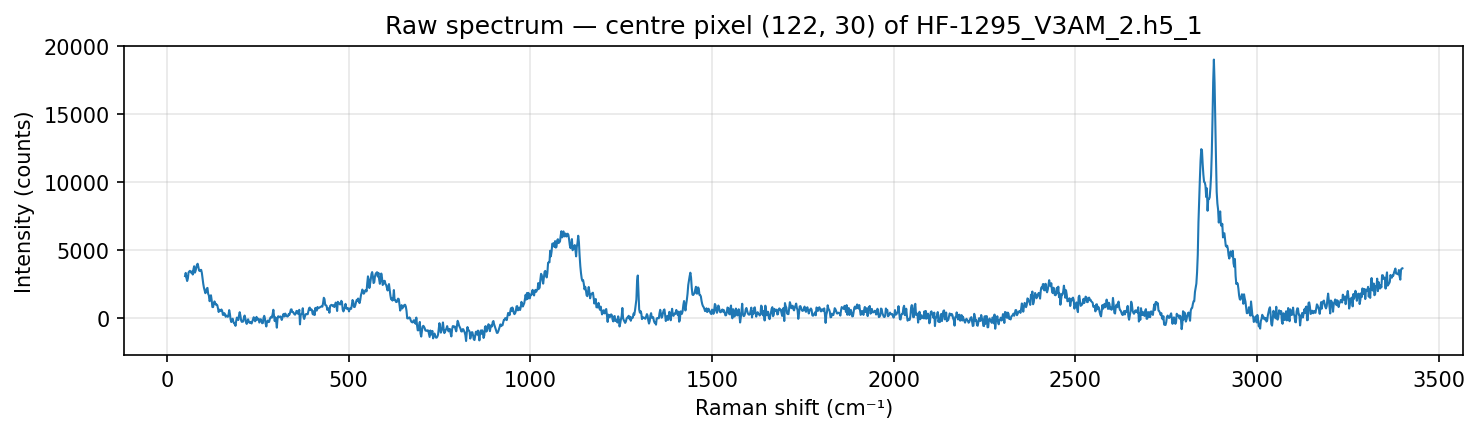
\includegraphics[width=\linewidth]{images/raw_spectrum_HF-1295_V3AM_2.h5_1.png}
    \caption{\footnotesize One raw spectrum of a sample in our dataset.}
    \label{fig:raw_spectrum}
\end{figure}

\section{Raman Spectroscopy in Medical Diagnosis}
\label{sec:rs_medical}
Many studies have been performed with RS in Medical Diagnosis, especially in oncology for tumor detection \cite{stupak2025raman,Auner2018}. However, given the high variability of protocols of using RS, and for lack of any standard protocol, results vary across study and are difficult to compare. Some examples of Raman protocols or techniques are: raw sample, frozen section, Surface Enhanced Raman Spectroscopy, Tip Enhanced Raman Spectroscopy, Resonance Raman Scattering, Surface Enhanced Resonance Raman Scattering, Spatially offset Raman Spectroscopy, Transmission Raman Spectroscopy, Coherent Anti-Stokes Raman Scattering, and Stimulated Raman Scattering \cite{Auner2018}.

RS produces raw spectra that are difficult or even impossible to interpret directly, therefore the standard approach in RS is to apply Machine Learning (ML) tools to map spectra to labels, as mapping the Raman spectrum to a chemical mixture of components is unfeasible, and often times impossible, especially for biological samples 
\cite{Boateng2025ramanmix}. This approach poses some difficulties in adoption of the method in medicine, as the models may not always be easily interpretable. However, given the high number of studies with promising results, it is possible that RS will be adopted in medicine in some form.

\TODO{A paragraph on the state of the ML side of the field, drawing on Sineesh and Kamsali \cite{sineesh2026raman}, who benchmark deep learning models for RS across open-source datasets and report four problems that recur regardless of application domain: (i) datasets are small; (ii) synthetic data is used extensively, but with unclear benefit in real-world application; (iii) there are few benchmarks, and deep models are seldom compared against classical ML or computer-vision baselines; and (iv) cross-paper performance comparison is difficult. State these in this general form here, since they frame every specific number quoted later: point (i) motivates the augmentation strategy of this work, point (ii) is precisely the question this thesis sets out to answer for glioma RS, point (iii) is why four downstream classifiers are evaluated rather than one, and point (iv) is why Table~\ref{tab:rs_brain_performance} reports validation schemes alongside accuracies. Note the pleasing symmetry: the field-wide critique in (ii) is what Chapter~\ref{sec:discussion} ends up confirming on this dataset.}



\subsection*{Reported performance in brain tumour applications}

\TODO{Write the prose around Table~\ref{tab:rs_brain_performance}; the numbers, cohorts and
validation schemes in it are taken from the three surveys and need no further checking. The
argument to build, in four moves:

(1) \emph{RS separates tumour from normal brain very well.} Reported accuracies cluster in
the 83--99\% range, and a meta-analysis over 1951 spectra puts glioma-vs-normal at 96\%
sensitivity / 99\% specificity. This is the result that motivates the whole field.

(2) \emph{Molecular classification is harder, and IDH status is the specific case this thesis
addresses.} Three groups report 87--89\% accuracy for IDH-mutant vs.\ IDH-wildtype, and
Livermore et al.\ report 91\% sensitivity / 95\% specificity. Note that the finer the
molecular distinction, the worse it gets: Galli et al.\ separate tumour from normal at
94--100\% but IDH-mutant oligodendroglioma from astrocytoma at only 81\%, and Zhou et al.\
fall from 99.6\% (glioma vs.\ normal) to 84.1\% (low- vs.\ high-grade) to 75.1\% overall on a
three-class problem. That degradation with granularity is the same pattern this work observes
between the binary task (Table~\ref{tab:binary_results}) and the six-class task
(Table~\ref{tab:sixclass_results}), and it is worth saying so explicitly.

(3) \emph{Cohorts are small.} The last column of Table~\ref{tab:rs_brain_performance} is the
one to dwell on: most studies work with fewer than 70 patients, several with fewer than 20.
The 58 slides used here are unremarkable for this literature -- which is the point, and the
motivation for the augmentation strategy of Section~\ref{sec:synthetic_rs}.

(4) \emph{Validation schemes differ enough to make the headline numbers hard to compare, and
this thesis's are conservative.} Most of these studies validate with leave-one-out or $k$-fold
cross-validation over \emph{spectra}, which places spectra from the same patient on both sides
of the split; a handful (Livermore et al., Riva et al.) use leave-one-patient-out. Under
patient-level validation the numbers fall: Riva et al.\ report 83\% for the comparatively easy
tumour-vs-normal task using random forests and gradient boosting -- the same model families
used here. Reading the $\sim$74\% of Table~\ref{tab:binary_results} against the 87--89\% IDH
figures without noting this difference would be misleading, and the honest comparison is the
one against Riva et al.\ and Livermore et al.

Be careful with attribution: these are three surveys, and Table~\ref{tab:rs_brain_performance}
credits the primary studies by name. If you want to cite the primary work directly rather
than the surveys, the DOIs are in the surveys' reference lists; as written, the table cites
the surveys, which is defensible for a background section.}

\begin{table}[htp]
\centering
\scriptsize
\caption{Reported performance of Raman spectroscopy in brain tumour applications, as collated
by three recent surveys \cite{hollon2021raman, murugappan2023raman, stupak2025raman}.
Grouped by task. Accuracy (Acc.), sensitivity (Sens.) and specificity (Spec.) in per cent;
a dash marks a figure the surveys do not report.}
\label{tab:rs_brain_performance}
\begin{tabular}{@{}p{3.3cm}p{3.1cm}p{2.2cm}>{\centering\arraybackslash}p{1.3cm}>{\centering\arraybackslash}p{1.2cm}>{\centering\arraybackslash}p{1.2cm}@{}}
\toprule
\emph{Study} & \emph{Cohort} & \emph{Validation} & \emph{Acc.} & \emph{Sens.} & \emph{Spec.}\\
\midrule
\multicolumn{6}{l}{\emph{Molecular / genetic classification}}\\
\midrule
Uckermann et al. & 36 froz. sect. & 5 bands, Mahal. & $89$ & -- & --\\
Sciortino et al. & fresh, post-resection & -- & $87$ & -- & --\\
Livermore et al. (IDH only) & 62 patients & LOPOCV & -- & $91$ & $95$\\
Livermore et al. (3 subtypes) & 62 patients & LOPOCV & -- & $79$--$94$ & $90$--$100$\\
Galli et al. (IDH-mut subtypes vs.\ astro) & 209 samples & PCA & $81$ & -- & --\\
\midrule
\multicolumn{6}{l}{\emph{Tumour vs.\ normal brain}}\\
\midrule
Zhang et al. (meta-analysis) & 1951 spectra & -- & -- & $96$ & $99$\\
Zhou et al. (VRRS) & -- & CV & $99.6$ & $100$ & $96.3$\\
Kalkanis et al. & frozen sections & -- & $97.8$ & -- & --\\
Iturrioz et al. & 4 patients & PCA-LDA & $92.5$ & -- & --\\
Jermyn et al. (\emph{in vivo}) & 17 pat., 161 spectra & LOOCV & $92$ & $93$ & $91$\\
Li et al. (KDE augment.) & 205 gl. / 37 norm. & -- & $91.67$ & $91.67$ & $91.67$\\
Riva et al. & 63 samples, 3450 spectra & LOPOCV, RF/GB & $83$ & -- & --\\
\midrule
\multicolumn{6}{l}{\emph{Grading}}\\
\midrule
Galli et al. (per subtype) & 209 samples & PCA & $86$--$100$ & -- & --\\
Zhou et al. (low vs.\,\ high grade) & -- & CV & $84.1$ & $96.3$ & $53.7$\\
Zhou et al. (normal / LGG / malignant) & -- & CV & $75.1$ & -- & --\\
Auner et al. (paediatric) & 64 samp., 28 pat. & PCA-DFA & $88.9$--$95.1$ & -- & --\\
\midrule
\multicolumn{6}{l}{\emph{Stimulated Raman histology (imaging, for context)}}\\
\midrule
Hollon et al. (SRH + CNN) & 278 patients & prosp. trial & $94.6$ & -- & --\\
Hollon et al. (H\&E comparator) & 278 patients & prosp. trial & $93.9$ & -- & --\\
Orringer et al. (SRH vs.\ H\&E) & 101 patients & $\kappa > 0.89$ & $>90$ & -- & --\\
\bottomrule
\end{tabular}
\small{LOOCV: leave-one-out cross-validation. LOPOCV: leave-one-patient-out cross-validation.
RF: random forest. GB: gradient boosting. VRRS: visible resonance Raman spectroscopy.
KDE: kernel density estimation. Note that only the LOPOCV entries guarantee that spectra from
one patient do not appear on both sides of the split; the remaining entries validate over
spectra, and their figures are correspondingly optimistic as estimates of performance on an
unseen patient.}
\end{table}

\subsection*{The study this dataset comes from}

\TODO{One or two paragraphs on Lita et al.\ \cite{apollonov2024raman}. This study is currently
mentioned only in passing in Chapter~\ref{sec:results}'s methodology, yet it supplies the
dataset, the labels, and the cross-validation design this work replicates -- it deserves to be
introduced properly here. Cover: what they set out to show (metabolic differences between
IDH-mutant and IDH-wildtype glioma detectable by RS), their preprocessing and tissue-selection
approach (PCA followed by DBSCAN over all spectra, which Section~\ref{sec:preprocessing_steps}
departs from and should justify departing from), the classifier they used (the RF+SVM
combination that appears here as one of the four downstream models), and the results they
reported. Then state plainly what this thesis adds on top: the generative augmentation, the
slide-level bootstrap, and the CbR inference strategy.}

\TODO{Optional but valuable: expand the existing paragraph on protocol heterogeneity. It
currently lists ten Raman variants in a single sentence and then asserts that results are hard
to compare. Say concretely why -- different excitation wavelengths, integration times,
normalisation choices and baseline-correction methods change the recorded spectrum, so a model
trained on one instrument's output does not transfer. This is the same instrument-variability
argument the introduction makes, and it motivates the augmentation strategy of this work.}


\section{Glioma Grading and Molecular Classification}
\label{sec:glioma_grading}

\TODO{This section does not yet exist and is the largest gap in this chapter. The thesis
classifies spectra into LGm1--LGm6 and into IDH-mutant vs.\ IDH-wildtype, but nowhere explains
where those categories come from or why they matter -- the labels are introduced in
Section~\ref{sec:data_collection} as a fait accompli. A reader should not have to take the
target variable on faith. Cover, in roughly this order:

(1) \emph{Clinical grading.} How gliomas are graded histopathologically, and the shift in the
WHO classification towards molecular rather than purely morphological criteria. Already cited
in the introduction: \texttt{whitfield2022classificationgliomas}. Note the turnaround time of
histopathology, since the case for RS in the introduction rests on it.

(2) \emph{IDH status.} What a mutation in isocitrate dehydrogenase does metabolically, why it
defines a prognostically distinct disease, and -- the point that matters here -- why the
resulting metabolic shift is large enough to leave a Raman signature. This is the biological
justification for the binary task being the easier of the two, an asymmetry the results
consistently show.

(3) \emph{The LGm methylation clusters.} Where LGm1--LGm6 come from: the pan-glioma DNA
methylation clustering of Ceccarelli et al.\ \cite{Ceccarelli2016}. State how the six clusters
map onto IDH status (LGm1--LGm3 mutant, LGm4--LGm6 wildtype), which is the grouping used
throughout this work. Then make the point that governs the 6-class results: methylation
subtypes are epigenetic distinctions, several steps removed from the molecular composition a
Raman spectrum measures, so there is no guarantee they are spectrally separable at all. The
~30\% 6-class accuracy in Section~\ref{sec:results_6class} is better read against that
expectation than against the binary result.

(4) \emph{Class imbalance as a clinical fact.} LGm1 and LGm6 are rare, which is why
Table~\ref{tab:dataset} is so uneven and why the cross-validation design of
Section~\ref{sec:cv_design} cannot be a clean partition. Worth stating here so that design
choice reads as forced rather than arbitrary.}

\section{Synthetic data for Raman Spectroscopy}
\label{sec:synthetic_rs}
Data augmentation is a comon technique used especially for Deep Learning (DL) models. In the context of RS, classic data augmentation techniques include (i) spectral shift, simulating instrument calibration drift, (ii) linear interpolation of spectra of the same class, or Synthetic Minority Over-sampling Technique (SMOTE), (iii) peak intensity perturbations \cite{zhao2024raman}.

A better approach involves learning the data distribution and constructing a generator of synthetic data. 

Evaluating such a data generator can be difficult, as we would like a quantitative measure of the data generator. Since a quantitative measure on the data itself may not be relevant for a particular task, the methodology of Train Real/Test Real vs. Train Synthetic/Test real was proposed \cite{esteban2017real}, where one trains a classifier on a real data train set, tests on a real data test set; the synthetic data generator is modeled on the train set, such that there is no data leakege from the test set via the generator. The same classifiers are then trained on synthetic data only, and tested on the same real data test set. This setup allows for quantitative measurements of the generator, as the training dataset can be compared against the synthetic data set. Any metric can be compared between the two models, such as accuracy, precision, recall, sensitivity, specificity.

A study of particular interest regarding synthetic data augmentation for RS in medical context was performed by Zhao et al. \cite{zhao2024raman} on in vivo skin cancer classification. They used a dataset of 731 spectra from 644 patients with 340 samples corresponding to cancerous and 391 corresponding to benign samples. They trained a 1D Generative Adversarial Network (GAN) on this data set and reported consistent improvements in accuracy in the range of 2-4\% across all classification models. Their findings suggest that deep generative data augmentation can help improve classification models.

\subsection*{Learned generative models for spectra}

\TODO{Half a page. The current text says only that "a better approach involves learning the
data distribution and constructing a generator" and then jumps straight to a single GAN study.
Fill in the families and what distinguishes them:
(i) GANs -- adversarial training, strong sample fidelity, but unstable to train and prone to
mode collapse, which is the failure mode this thesis observes in a VAE guise (the narrow
$\sigma$ envelope of Figure~\ref{fig:mean_std_spectra});
(ii) VAEs -- explicit likelihood bound, stable training, an interpretable latent space, at the
cost of blurrier / lower-variance samples. State plainly that this is the trade-off motivating
the choice made in this work, and forward-reference Section~\ref{sec:cvae};
(iii) diffusion models -- currently named in the future-work paragraph of
Chapter~\ref{sec:discussion} without ever having been introduced, which should be fixed here
even if only in two sentences.
Directly relevant entries already in the bibliography and uncited: \texttt{Gebran2025}
(conditional VAEs generating stellar spectra -- the closest published analogue to what this
work does, a CVAE generating 1-D spectra) and \texttt{Kavran2022} ($\beta$-VAE augmentation
for time-series classification, which is the same architecture class applied to the same kind
of sequential signal).}

\subsection*{Evaluating a generator}

\TODO{Extend the existing TS/TR paragraph, which covers the protocol but not what a generator
can fail at. The standard framing is three-way and worth stating explicitly, because this
thesis's results separate along exactly these axes:
(i) \emph{fidelity} -- are samples individually realistic? Here: yes, the mean spectra match
closely (Figure~\ref{fig:mean_std_spectra});
(ii) \emph{diversity} -- do samples cover the real distribution's spread? Here: no, and this
is the central negative finding;
(iii) \emph{privacy} -- do samples memorise training data? Relevant to the clinical
data-sharing motivation and worth a sentence even though this thesis does not measure it.
Uncited entry available: \texttt{jordon2022synthetic}. Note that a generator can score well on
a TS/TR classifier metric while failing (ii) badly, which is precisely the pattern in
Table~\ref{tab:binary_results} -- RF reaches 0.669 under TS/TR from a distribution far
narrower than the real one.}
